% ----------------------------------------------------------------------
\section{Subspaces and basis}

% ----------------------------------------------------------------------
\subsection{Definition of subspace}

As we saw earlier, the span of 0 vectors in $\R^n$ is a point, namely
the set $\set{\vect{0}}$. The span of one non-zero vector is a line
through the origin, and the span of two linearly independent vectors
is a plane through the origin.
\begin{center}
  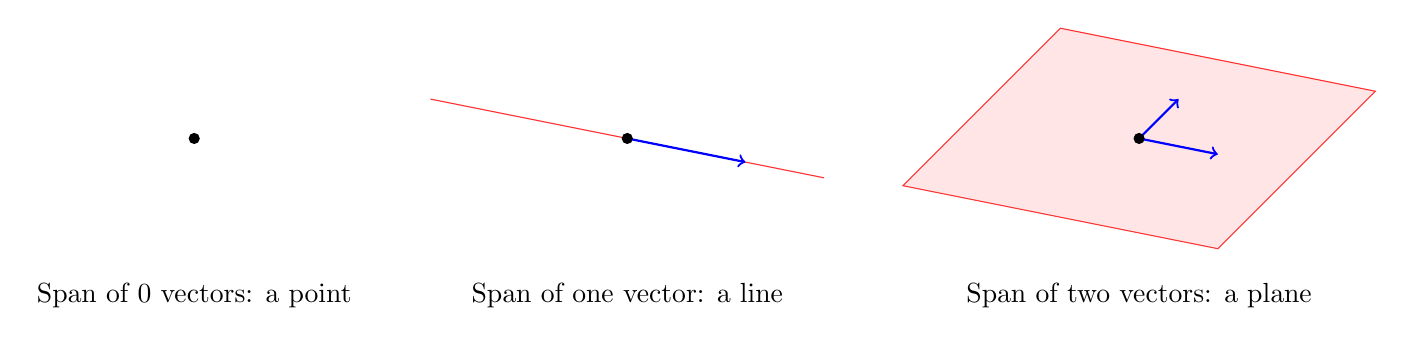
\begin{tikzpicture}
    \begin{scope}[xshift=-6cm]
      \draw[fill](0,0) circle [radius=1.8pt];
      \path(0,-2) node {Span of 0 vectors: a point};
    \end{scope}
    \begin{scope}[xshift=-0.5cm]
      \begin{scope}[x={(1cm,-0.2cm)},y={(0.5cm,0.5cm)}]
        \draw[red!80](-2.5,0) -- (2.5,0);
        \draw[->, thick, blue](0,0) -- +(1.5,0);
        \draw[fill](0,0) circle [radius=1.8pt];
      \end{scope}
      \path(0,-2) node {Span of one vector: a line};
    \end{scope}
    \begin{scope}[xshift=6cm]
      \begin{scope}[x={(1cm,-0.2cm)},y={(0.5cm,0.5cm)},z={(0cm,1cm)}]
        \filldraw[draw=red!80,fill=red!10](-2,-2,0) -- (2,-2,0) -- (2,2,0) -- (-2,2,0) -- cycle;
        \draw[->, thick, blue](0,0) -- +(0,1,0);
        \draw[->, thick, blue](0,0,0) -- +(1,0,0);
        \draw[fill](0,0) circle [radius=1.8pt];
      \end{scope}
      \path(0,-2) node {Span of two vectors: a plane};
    \end{scope}
  \end{tikzpicture}
\end{center}
We also call these sets, respectively, a {\em $0$-dimensional
  subspace}, a {\em $1$-dimensional subspace}, and a {\em
  $2$-dimensional subspace} of\/ $\R^n$. The purpose of this section is
to generalize this concept of subspace to arbitrary dimensions.

\begin{definition}{Subspace}{subspace}
  A subset $V$ of\/ $\R^n$ is called a \textbf{subspace}%
  \index{subspace!of Rn@of $\R^n$} of $\R^n$ if
  \begin{enumerate}
  \item $V$ contains the zero vector of\/ $\R^n$, i.e., $\vect{0}\in V$;
  \item $V$ is closed under addition, i.e., for all\/
    $\vect{u},\vect{w}\in V$, we have $\vect{u}+\vect{w}\in V$;
  \item $V$ is closed under scalar multiplication, i.e., for all\/
    $\vect{u}\in V$ and scalars $k$, we have\/ $k\,\vect{u}\in V$.
  \end{enumerate}
\end{definition}

Notice that the subset $V = \set{\vect{0}}$ is a subspace of $\R^n$
(called the \textbf{zero subspace}\index{zero subspace}%
\index{subspace!zero subspace}). Every line or plane through the
origin is a subspace. Moreover, the entire space $\R^n$ is a subspace
of itself. A subspace that is not the zero subspace or the entire
space $\R^n$ is referred to as a \textbf{proper subspace}%
\index{proper subspace}\index{subspace!proper} of $\R^n$.

% ----------------------------------------------------------------------
\subsection{Examples of subspaces}

\begin{proposition}{Spans are subspaces}{span-subspace}
  Let $\vect{u}_1,\ldots,\vect{u}_k$ be vectors in $\R^{n}$. Then
  $\sspan\set{\vect{u}_1,\ldots,\vect{u}_k}$ is a subspace of
  $\R^{n}$.%
  \index{subspace!span is a subspace}%
  \index{span!as a subspace}%
  \index{vector!span!as a subspace}%
\end{proposition}

\begin{proof}
  Let $S=\sspan\set{\vect{u}_1,\ldots,\vect{u}_k}$. To verify that $S$
  is a subspace of $\R^{n}$, we must check that the three conditions
  of Definition~\ref{def:subspace} hold.
  \begin{itemize}
  \item We have $\vect{0}\in S$ because
    $\vect{0}=0\vect{u}_1+\ldots+0\vect{u}_k$. 
  \item Suppose $\vect{u},\vect{w}\in S$.
    By definition of span, there exist scalars $a_1,\ldots,a_k$ and
    $b_1,\ldots,b_k$ such that
    $\vect{u}=a_1\,\vect{u}_1+\ldots+a_k\,\vect{u}_k$ and
    $\vect{w}=b_1\,\vect{u}_1+\ldots+b_k\,\vect{u}_k$.
    Therefore,
    \begin{equation*}
      \vect{u}+\vect{w} = \vect{u}=(a_1+b_1)\vect{u}_1+\ldots+(a_k+b_k)\vect{u}_k.
    \end{equation*}
    It follows that
    $\vect{u}+\vect{w}\in S=\sspan\set{\vect{u}_1,\ldots,\vect{u}_k}$,
    so that $S$ is closed under addition.
  \item Suppose $\vect{u}\in S$ and $t$ is a scalar. Then by
    definition of span, there exists scalars $a_1,\ldots,a_k$ such
    that $\vect{u}=a_1\,\vect{u}_1+\ldots+a_k\,\vect{u}_k$. Then
    \begin{equation*}
      t\,\vect{u}=(ta_1)\vect{u}_1+\ldots+(ta_k)\vect{u}_k,
    \end{equation*}
    and thus $t\,\vect{u}\in S$. It follows that $S$ is closed under
    scalar multiplication.
  \end{itemize}
  Since $S=\sspan\set{\vect{u}_1,\ldots,\vect{u}_k}$ satisfies all
  three conditions, it follows that it is a subspace of $\R^n$.
\end{proof}

\begin{example}{A line in $\R^3$}{line-subspace}
  In $\R^3$, let $L$ be the line through the origin that is
  parallel to the vector
  \begin{equation*}
    {\vect{d}}= \begin{mymatrix}{r} -5 \\ 1 \\ -4 \end{mymatrix}.
  \end{equation*}
  Show that $L$ is a subspace of $\R^3$.
\end{example}

\begin{solution}
  The line $L$ is simply the span of the vector $\vect{d}$, i.e.,
  $L=\sspan\set{\vect{d}}$. Therefore, it is a subspace by
  Proposition~\ref{prop:span-subspace}.
\end{solution}

\begin{proposition}{Solution space of a homogeneous system of equations}{solution-space}
  Consider a homogeneous system of equations $A\vect{x} = \vect{0}$,
  where $A$ is an $m\times n$-matrix. Then the set of solutions,
  \begin{equation*}
    V=\set{\vect{x}\in\R^n \mid A\vect{x} = \vect{0}},
  \end{equation*}
  is a subspace of $\R^n$. It is called the \textbf{solution space} of
  the system.%
  \index{subspace!solution space of a homogeneous system}%
  \index{homogeneous system!solution space}%
  \index{solution space}%
  \index{system of linear equations!homogeneous!solution space}%
  \index{system of linear equations!solution space}
\end{proposition}

\begin{proof}
  To show that $V$ is a subspace of $\R^{n}$, we check the three
  conditions of Definition~\ref{def:subspace}.
  \begin{itemize}
  \item We have $\vect{0}\in V$ because $A\vect{0}=\vect{0}$.
  \item To show that $V$ is closed under addition, suppose
    $\vect{u},\vect{w}\in V$.  Then by definition of $V$,
    $A\vect{u}=\vect{0}$ and $A\vect{w}=\vect{0}$.  Therefore,
    \begin{equation*}
      A(\vect{u}+\vect{w}) = A\vect{u} + A\vect{w} = \vect{0}+\vect{0}
      = \vect{0}.
    \end{equation*}
    It follows that $\vect{u}+\vect{w}\in V$.
  \item To show that $V$ is closed under scalar multiplication,
    suppose $\vect{u}\in V$ and $t$ is a scalar. Then by definition of
    $V$, we have $A\vect{u}=\vect{0}$. It follows that 
    \begin{equation*}
      A(t\,\vect{u}) = t(A\vect{u}) = t\,\vect{0} = \vect{0}.
    \end{equation*}
    Therefore, $t\,\vect{u}\in V$.
  \end{itemize}
  Since the solution space
  $V=\set{\vect{x}\in\R^n \mid A\vect{x} = \vect{0}}$ satisfies all
  three conditions, it is a subspace of $\R^n$.
\end{proof}

\begin{example}{A plane in $\R^3$}{plane-subspace}
  Show that the plane $2x+3y-z=0$ is a subspace of $\R^3$.
\end{example}

\begin{solution}
  Since $2x+3y-z=0$ is a homogeneous equation, its solution space
  \begin{equation*}
    \set{\left.\begin{mymatrix}{c}x\\y\\z\end{mymatrix}~\right\vert~ 2x+3y-z=0}
  \end{equation*}
  is a subspace of $\R^3$ by Proposition~\ref{prop:solution-space}.
\end{solution}

\begin{example}{Non-examples}{subspace-non-examples}
  Which of the following are subspaces of $\R^3$?
  \begin{enumialphparenastyle}
    \begin{enumerate}
    \item The line
      \begin{equation*}
        \begin{mymatrix}{c}x\\y\\z\end{mymatrix}
        = \begin{mymatrix}{c}1\\2\\3\end{mymatrix}
        + t\begin{mymatrix}{c}1\\0\\1\end{mymatrix}.
      \end{equation*}
    \item The plane $2x+3y-z=5$.
    \item The set of vectors
      \begin{equation*}
        W=\set{\left.\begin{mymatrix}{c}x\\y\\z\end{mymatrix}
            ~\right\vert~ x,y,z\geq 0}.
      \end{equation*}
      ~
    \end{enumerate}
  \end{enumialphparenastyle}
\end{example}

\begin{solution}
  None of them are subspaces. Neither the line (a) nor the plane (b)
  contains the origin $\vect{0}$, so they fail to satisfy the first
  condition of subspaces. The set of vectors in (c) contains
  $\vect{0}$. It is also closed under addition. However, it fails to
  be closed under scalar multiplication. For example, let
  $\vect{u}=\mat{1,1,1}^T$. Then $\vect{u}\in W$, but
  $(-1)\vect{u}\not\in W$.
\end{solution}

% ----------------------------------------------------------------------
\subsection{Definition of basis}

We saw in Proposition~\ref{prop:span-subspace} that spans are
subspaces of $\R^n$. Interestingly, the converse is also true: every
subspace of $\R^n$ is the span of some finite set of vectors.

\begin{theorem}{Subspaces are spans}{subspaces-are-spans}
  Let $V$ be a subspace of\/ $\R^n$. Then there exist linearly
  independent vectors $\set{\vect{u}_{1},\ldots,\vect{u}_{k}}$ in $V$
  such that
  \begin{equation*}
    V= \sspan\set{\vect{u}_{1},\ldots ,\vect{u}_{k}}. 
  \end{equation*}%
  \index{subspace!subspace is a span}
  \vspace{-3ex}
\end{theorem}

\begin{proof}
  We proceed as follows.
  \begin{enumerate}
  \item[0.] If $V=\set{\vect{0}}$, then $V$ is the empty span, and we
    are done.
  \item[1.] Otherwise, $V$ contains some non-zero vector.  Pick a
    non-zero vector $\vect{u}_{1}$ in $V$. If
    $V=\sspan\set{\vect{u}_{1}}$, we are done.
  \item[2.] Otherwise, pick a vector $\vect{u}_{2}$ in $V$ that is not
    in $\sspan\set{\vect{u}_{1}}$. If
    $V=\sspan\set{\vect{u}_{1},\vect{u}_{2}}$, we are done.
  \item[3.] Otherwise, pick a vector $\vect{u}_{3}$ in $V$ that is not
    in $\sspan\set{\vect{u}_{1},\vect{u}_{2}}$. If
    $V=\sspan\set{\vect{u}_{1},\vect{u}_{2},\vect{u}_{3}}$, we are done.
  \item[4.] Otherwise, pick a vector $\vect{u}_{4}$ in $V$ that is not
    in $\sspan\set{\vect{u}_{1},\vect{u}_{2},\vect{u}_{4}}$, and so on.
  \end{enumerate}
  Continue in this way. Note that after the $j\th$ step of this
  process, the vectors $\vect{u}_1,\ldots,\vect{u}_j$ are linearly
  independent. This is because, by construction, no vector is in the
  span of the previous vectors, and therefore no vector is redundant.
  By
  Theorem~\ref{thm:properties-linear-independence}(\ref{properties-linear-independence-c}),
  there can be at most $n$ linearly independent vectors in $\R^n$.
  Therefore the process must stop after $k$ steps for some $k\leq
  n$. But then $V=\sspan\set{\vect{u}_{1},\ldots ,\vect{u}_{k}}$, as
  desired.
\end{proof}

In summary, every subspace of $\R^{n}$ is spanned by a finite,
linearly independent collection of vectors.  Such a collection of
vectors is called a \textbf{basis} of the subspace.

\begin{definition}{Basis of a subspace}{subspace-basis}
  Let $V$ be a subspace of $\R^{n}$. Then
  $\set{\vect{u}_{1},\ldots ,\vect{u}_{k}}$ is a \textbf{basis} for
  $V$ if the following two conditions hold:%
  \index{basis}%
  \index{subspace!basis|see{basis}}%
  \index{vector!basis|see{basis}}%
  \begin{enumerate}
  \item $\sspan\set{\vect{u}_{1},\ldots,\vect{u}_{k}}=V$, and
  \item $\vect{u}_{1},\ldots,\vect{u}_{k}$ are linearly independent.
  \end{enumerate}
\end{definition}

Note that the plural of basis is \textbf{bases}.

% ----------------------------------------------------------------------
\subsection{Examples of bases}

\begin{proposition}{Standard basis of $\R^n$}{standard-basis}
  Let $\vect{e}_i$ be the vector in $\R^n$ whose $i\th$ entry is $1$
  and all of whose other entries are $0$. In other words, $\vect{e}_i$
  is the $i\th$ column of the identity matrix.
  \begin{equation*}
    \vect{e}_1 = \begin{mymatrix}{c}1\\0\\0\\\vdots\\0\end{mymatrix},\quad
    \vect{e}_2 = \begin{mymatrix}{c}0\\1\\0\\\vdots\\0\end{mymatrix},\quad
    \vect{e}_3 = \begin{mymatrix}{c}0\\0\\1\\\vdots\\0\end{mymatrix},\quad
    \ldots~,\quad
    \vect{e}_n = \begin{mymatrix}{c}0\\0\\0\\\vdots\\1\end{mymatrix}.
  \end{equation*}
  Then $\set{\vect{e}_1,\vect{e}_2,\ldots,\vect{e}_n}$ is a basis for
  $\R^n$. It is called the \textbf{standard basis}%
  \index{standard basis}%
  \index{basis!standard}
  of $\R^n$.
\end{proposition}

\begin{proof}
  To see that it is a basis of $\R^n$, first notice that the vectors
  $\vect{e}_1,\vect{e}_2,\ldots,\vect{e}_n$ span $\R^n$. Indeed, every
  vector $\vect{v} = \mat{x_1,\ldots,x_n}^T\in\R^n$ can be written as
  $\vect{v} = x_1\vect{e}_1+\ldots+x_n\vect{e}_n$. Second, the vectors
  $\vect{e}_1,\vect{e}_2,\ldots,\vect{e}_n$ are evidently linearly
  independent, because none of these vectors can be written as a
  linear combination of previous vectors. Since the vectors span
  $\R^n$ and are linearly independent, they form a basis of $\R^n$.
\end{proof}

\begin{example}
  Check that the vectors
  \begin{equation*}
    \vect{v}_1 = \begin{mymatrix}{r}1\\2\\1\end{mymatrix},\quad
    \vect{v}_2 = \begin{mymatrix}{r}0\\1\\0\end{mymatrix},\quad
    \mbox{and}\quad
    \vect{v}_3 = \begin{mymatrix}{r}1\\0\\-1\end{mymatrix}
  \end{equation*}
  form a basis of $\R^3$.
\end{example}

\begin{solution}
  ...........
\end{solution}

% ======================================================================
\subsection{CONTINUE HERE}

The following is a simple but very useful example of a basis, called
the standard basis.

\begin{definition}{Standard basis of $\R^n$}{standard-basis}
\end{definition}

The main theorem about bases is not only they exist, but that they
must be of the same size. To show this, we will need the the following
fundamental result, called the Exchange Theorem.

\begin{theorem}{Exchange theorem}{exchange-theorem}
  Suppose $\set{\vect{u}_{1},\ldots ,\vect{u}_{r}} $ is a linearly
  independent set of vectors in $\R^n$, and each $\vect{u}_{k}$ is
  contained in $\sspan\set{\vect{v}_{1},\ldots
    ,\vect{v}_{s}}$ Then $s\geq r$. \\
  In words, spanning\index{exchange theorem} sets have at least as
  many vectors as linearly independent sets.
\end{theorem}

\begin{proof}
  Since each $\vect{u}_j$ is in
  $\sspan\set{\vect{v}_{1},\ldots ,\vect{v}_{s}} $, there exist
  scalars $a_{ij}$ such that
  \begin{equation*}
    \vect{u}_{j}=\sum_{i=1}^{s}a_{ij}\vect{v}_{i}
  \end{equation*}
  Suppose for a contradiction that $s<r$. Then the matrix
  $A = \mat{ a_{ij} }$ has fewer rows, $s$ than columns, $r$. Then the
  system $AX=0$ has %Theorem~\ref{thm:rank-homogeneous-solutions}
  a non-trivial solution $\vect{d}$, that is there is a
  $\vect{d}\neq \vect{0}$ such that $A\vect{d}=\vect{0}$. In other
  words,
  \begin{equation*}
    \sum_{j=1}^{r}a_{ij}d_{j}=0,\;i=1,2,\ldots ,s
  \end{equation*}
  Therefore, 
  \begin{eqnarray*}
    \sum_{j=1}^{r}d_{j}\vect{u}_{j}
    &=&\sum_{j=1}^{r}d_{j}\sum_{i=1}^{s}a_{ij}
        \vect{v}_{i} \\
    &=&\sum_{i=1}^{s}\tup{\sum_{j=1}^{r}a_{ij}d_{j}} \vect{v}
        _{i}=\sum_{i=1}^{s}0\vect{v}_{i}=0
  \end{eqnarray*}
  which contradicts the assumption that
  $\set{\vect{u}_{1},\ldots ,\vect{u}_{r}} $ is linearly independent,
  because not all the $d_{j}$ are zero. Thus this contradiction
  indicates that $s\geq r$.
\end{proof}

We are now ready to show that any two bases are of the same size.

\begin{theorem}{Bases of $\R^{n}$ are of the same size}{bases-same-size}
  Let $V$ be a subspace of $\R^{n}$ with two bases $B_1$ and
  $B_2$. Suppose $B_1$ contains $s$ vectors and $B_2$ contains $r$
  vectors. Then $s=r$.
\end{theorem}

\begin{proof}
  This follows right away from
  Theorem~\ref{thm:exchange-theorem}. Indeed observe that
  $B_1 = \set{ \vect{u}_{1},\ldots ,\vect{u}_{s}} $ is a spanning set
  for $V$ while $ B_2 = \set{\vect{v}_{1},\ldots ,\vect{v}_{r}} $ is
  linearly independent, so $s \geq r$. Similarly
  $B_2 = \set{\vect{v}_{1},\ldots ,\vect{v} _{r}} $ is a spanning set
  for $V$ while $B_1 = \set{\vect{u}_{1},\ldots , \vect{u}_{s}} $ is
  linearly independent, so $r\geq s$.
\end{proof}

The following definition can now be stated.

\begin{definition}{Dimension of a subspace}{dimension}
  Let $V$ be a subspace of $\R^{n}$. Then the \textbf{dimension }of
  $V$, written $\func{dim}(V)$ is defined to be the number of vectors
  in a basis.\index{dimension}\index{subspace!dimension}
\end{definition}

The next result follows.

\begin{corollary}{Dimension of $\R^n$}{dimension-Rn}
  The dimension of $\R^{n}$ is $n$.
\end{corollary}

\begin{proof}
  You only need to exhibit a basis for $\R^{n}$ which has $n$
  vectors. Such a basis is the standard basis
  $\set{\vect{e}_{1},\ldots , \vect{e}_{n}}$.
\end{proof}

Consider the following example.

\begin{example}{Basis of subspace}{basis-subspace}
  Let 
  \begin{equation*}
    V=\set{
      \begin{mymatrix}{c} a\\ b\\ c\\ d\end{mymatrix}\in\R^4 \mid
      a-b=d-c
    }.
  \end{equation*}
  Show that $V$ is a subspace of $\R^4$, find a basis of $V$, and find
  $\dim(V)$.
\end{example}

\begin{solution}
  The condition $a-b=d-c$ is equivalent to the condition $a=b-c+d$, so
  we may write

  \begin{equation*}
    V =\set{
      \begin{mymatrix}{c} b-c+d\\ b\\ c\\ d\end{mymatrix} \mid b,c,d
      \in\R } = \set{ b\begin{mymatrix}{c} 1\\ 1\\ 0\\ 0\end{mymatrix}
      +c\begin{mymatrix}{c} -1\\ 0\\ 1\\ 0\end{mymatrix}
      +d\begin{mymatrix}{c} 1\\ 0\\ 0\\ 1\end{mymatrix} \mid b,c,d\in\R
    }
  \end{equation*}

  This shows that $V$ is a subspace of $\R^4$, since
  $V=\sspan\set{\vect{u}_1, \vect{u}_2, \vect{u}_3}$ where

  \begin{equation*}
    \vect{u}_1  =  \begin{mymatrix}{r} 1 \\ 1 \\ 0 \\ 0 \end{mymatrix},
    \vect{u}_2  =  \begin{mymatrix}{r} -1 \\ 0 \\ 1 \\ 0 \end{mymatrix}, 
    \vect{u}_3  =  \begin{mymatrix}{r} 1 \\ 0 \\ 0 \\ 1 \end{mymatrix}
  \end{equation*}

  Furthermore,

  \begin{equation*}
    \set{
      \begin{mymatrix}{c} 1\\ 1\\ 0\\ 0\end{mymatrix},
      \begin{mymatrix}{c} -1\\ 0\\ 1\\ 0\end{mymatrix},
      \begin{mymatrix}{c} 1\\ 0\\ 0\\ 1\end{mymatrix}
    }
  \end{equation*}
  is linearly independent, as can be seen by taking the
  {\rref} of the matrix whose columns are
  $\vect{u}_1, \vect{u}_2$ and $\vect{u}_3$.

  \begin{equation*}
    \begin{mymatrix}{rrr}
      1 & -1 & 1 \\
      1 & 0 & 0 \\
      0 & 1 & 0 \\
      0 & 0 & 1 \end{mymatrix}
    \rightarrow
    \begin{mymatrix}{rrr}
      1 & 0 & 0 \\
      0 & 1 & 0 \\
      0 & 0 & 1 \\
      0 & 0 & 0 \end{mymatrix}
  \end{equation*}
  
  Since every column of the {\rref} matrix has a leading one,
  the columns are linearly independent.

  Therefore $\set{\vect{u}_1, \vect{u}_2, \vect{u}_3}$ is linearly
  independent and spans $V$, so is a basis of $V$. Hence $V$ has
  dimension three.
\end{solution}

We continue by stating further properties of a set of vectors in
$\R^{n}$.

\begin{corollary}{Linearly independent and spanning sets in  $\R^{n}$}{independent-spanning-Rn}
  The following properties hold in $\R^{n}$:
  \begin{itemize}
  \item Suppose $\set{\vect{u}_{1},\ldots ,\vect{u}_{n}} $ is linearly
    independent. Then $\set{\vect{u}_{1},\ldots ,\vect{u}_{n}} $ is a
    basis for $\R^{n}$.
  \item Suppose $\set{\vect{u}_{1},\ldots ,\vect{u}_{m}} $ spans
    $\R^{n}$. Then $m\geq n$.
  \item If $\set{\vect{u}_{1},\ldots ,\vect{u}_{n}} $ spans $\R^{n}$,
    then $\set{\vect{u}_{1},\ldots ,\vect{u}_{n}} $ is linearly
    independent.
  \end{itemize}
\end{corollary}

\begin{proof}
  Assume first that $\set{\vect{u}_{1},\ldots ,\vect{u}_{n}} $ is
  linearly independent, and we need to show that this set spans
  $\R^{n}$. To do so, let $\vect{v}$ be a vector of $\R^{n}$, and we
  need to write $\vect{v}$ as a linear combination of $\vect{u}_i$'s.
  Consider the matrix $A$ having the vectors $\vect{u}_i$ as columns:
  \begin{equation*}
    A = 
    \begin{mymatrix}{rrr}
      \vect{u}_{1} & \ldots & \vect{u}_{n} 
    \end{mymatrix}
  \end{equation*}
  By linear independence of the $\vect{u}_i$'s, the {\rref} of $A$ is
  the identity matrix.  Therefore the system $A\vect{x}= \vect{v}$ has
  a (unique) solution, so $\vect{v}$ is a linear combination of the
  $\vect{u}_i$'s.

  To establish the second claim, suppose that $m<n$. Then letting
  $\vect{u}_{i_{1}},\ldots ,\vect{u}_{i_{k}}$ be the pivot columns of
  the matrix
  \begin{equation*}
    \begin{mymatrix}{ccc}
      \vect{u}_{1} & \ldots & \vect{u}_{m}
    \end{mymatrix}
  \end{equation*}
  it follows $k\leq m<n$ and these $k$ pivot columns would be a basis
  for $\R^{n}$ having fewer than $n$ vectors, contrary to
  Corollary~\ref{cor:dimension-Rn}.

  Finally consider the third claim. If $\set{\vect{u}_{1},\ldots
    ,\vect{u}_{n}} $ is not linearly independent, then replace this
  list with $\set{\vect{u}_{i_{1}},\ldots ,\vect{u}_{i_{k}}} $ where these
  are the pivot columns of the matrix 
  \begin{equation*}
    \begin{mymatrix}{ccc}
      \vect{u}_{1} & \ldots & \vect{u}_{n}
    \end{mymatrix}
  \end{equation*}
  Then $\set{\vect{u}_{i_{1}},\ldots ,\vect{u}_{i_{k}}} $ spans
  $\R^{n}$ and is linearly independent, so it is a basis having
  less than $n$ vectors again contrary to Corollary~\ref{cor:dimension-Rn}.
\end{proof}

The next theorem follows from the above claim.

\begin{theorem}{Existence of basis}{existence-basis}
  Let $V$ be a subspace of $\R^n$. Then there exists a basis of $V$ with 
  $\dim(V)\leq n$.
\end{theorem}

Consider Corollary~\ref{cor:independent-spanning-Rn} together with Theorem~\ref{thm:existence-basis}. Let $\dim(V) = r$. Suppose there exists an independent set of vectors in $V$. If this set contains $r$ vectors, then it is a basis for $V$. If it contains less than $r$ vectors, then vectors can be added to the set to create a basis of $V$. Similarly, any spanning set of $V$ which contains more than $r$ vectors can have vectors removed to create a basis of $V$.

We illustrate this concept in the next example.

\begin{example}{Extending an independent set}{extend-independent}
  Consider the set $U$ given by 
  \begin{equation*}
    U=\set{\left.\begin{mymatrix}{c} a\\ b\\ c\\ d\end{mymatrix}
        \in\R^4 \right\vert a-b=d-c
    }
  \end{equation*}
  Then $U$ is a subspace of $\R^4$ and $\dim(U)=3$.

  Then
  \begin{equation*}
    S=\set{
      \begin{mymatrix}{c} 1\\ 1\\ 1\\ 1\end{mymatrix},
      \begin{mymatrix}{c} 2\\ 3\\ 3\\ 2\end{mymatrix}
    },
  \end{equation*}
  is an independent subset of $U$.
  Therefore $S$ can be extended to a basis of $U$.
\end{example}

\begin{solution}
  To extend $S$ to a basis of $U$, find a vector in $U$ that is {\bf not} in
  $\sspan(S)$.
  \begin{equation*}
    \begin{mymatrix}{rrr}
      1 & 2 & ? \\
      1 & 3 & ? \\
      1 & 3 & ? \\
      1 & 2 & ? 
    \end{mymatrix}
  \end{equation*}

  \begin{equation*}
    \begin{mymatrix}{rrr}
      1 & 2 & 1 \\
      1 & 3 & 0 \\
      1 & 3 & -1 \\
      1 & 2 & 0 
    \end{mymatrix}
    \rightarrow
    \begin{mymatrix}{rrr}
      1 & 0 & 0 \\
      0 & 1 & 0 \\
      0 & 0 & 1 \\
      0 & 0 & 0 
    \end{mymatrix}
  \end{equation*}

  Therefore, $S$ can be extended to the following basis of $U$:
  \begin{equation*}
    \set{
      \begin{mymatrix}{r} 1\\ 1\\ 1\\ 1\end{mymatrix},
      \begin{mymatrix}{r} 2\\ 3\\ 3\\ 2\end{mymatrix},
      \begin{mymatrix}{r} 1\\ 0\\ -1\\ 0\end{mymatrix}
    },
  \end{equation*}
\end{solution}

Next we consider the case of removing vectors from a spanning set to
result in a basis.

\begin{theorem}{Finding a basis from a span}{}
  Let $W$ be a subspace. Also suppose that
  $W=\sspan\set{\vect{w} _{1},\ldots ,\vect{w}_{m}}$. Then there
  exists a subset of $\set{ \vect{w}_{1},\ldots ,\vect{w}_{m}} $ which
  is a basis for $W$.\index{spanning set!basis}
\end{theorem}

\begin{proof}
  Let $S$ denote the set of positive integers such that for $ k\in S$,
  there exists a subset of $\set{\vect{w}_{1},\ldots ,\vect{w}_{m}} $
  consisting of exactly $k$ vectors which is a spanning set for
  $W$. Thus $m\in S$. Pick the smallest positive integer in $S$. Call
  it $k$. Then there exists
  $\set{\vect{u}_{1},\ldots , \vect{u}_{k}} \subseteq
  \set{\vect{w}_{1},\ldots ,\vect{w} _{m}} $ such that
  $\sspan\set{\vect{u}_{1},\ldots ,\vect{u} _{k}} =W$. If
  \begin{equation*}
    \sum_{i=1}^{k}c_{i}\vect{w}_{i}=\vect{0}
  \end{equation*}
  and not all of the $c_{i}=0$, then you could pick $c_{j}\neq 0$,
  divide by it and solve for $\vect{u}_{j}$ in terms of the others,
  \begin{equation*}
    \vect{w}_{j}=\sum_{i\neq j}\tup{-\frac{c_{i}}{c_{j}}} \vect{w}_{i}
  \end{equation*}
  Then you could delete $\vect{w}_{j}$ from the list and have the same
  span. Any linear combination involving $\vect{w}_{j}$ would equal
  one in which $\vect{w}_{j}$ is replaced with the above sum, showing
  that it could have been obtained as a linear combination of
  $\vect{w}_{i}$ for $i\neq j$. Thus $k-1\in S$ contrary to the choice
  of $k$ . Hence each $c_{i}=0$ and so
  $\set{\vect{u}_{1},\ldots ,\vect{u} _{k}} $ is a basis for $W$
  consisting of vectors of $\set{\vect{w} _{1},\ldots ,\vect{w}_{m}}$.
\end{proof}

The following example illustrates how to carry out this shrinking
process which will obtain a subset of a span of vectors which is
linearly independent.

\begin{example}{Subset of a span}{subset-basis}
  Let $W$ be the subspace 
  \begin{equation*}
    \sspan\set{\begin{mymatrix}{r} 1 \\ 2 \\ -1 \\ 1 \end{mymatrix},
      \begin{mymatrix}{r} 1 \\ 3 \\ -1 \\ 1 \end{mymatrix},
      \begin{mymatrix}{r} 8 \\ 19 \\ -8 \\ 8 \end{mymatrix},
      \begin{mymatrix}{r} -6 \\ -15 \\ 6 \\ -6 \end{mymatrix},
      \begin{mymatrix}{r} 1 \\ 3 \\ 0 \\ 1 \end{mymatrix},
      \begin{mymatrix}{r} 1 \\ 5 \\ 0 \\ 1 \end{mymatrix}
    }
  \end{equation*}
  Find a basis for $W$ which consists of a subset of the given
  vectors.
\end{example}

\begin{solution}
  You can use the {\rref} to accomplish this reduction. Form
  the matrix which has the given vectors as columns. 
  \begin{equation*}
    \begin{mymatrix}{rrrrrr}
      1 & 1 & 8 & -6 & 1 & 1 \\ 
      2 & 3 & 19 & -15 & 3 & 5 \\ 
      -1 & -1 & -8 & 6 & 0 & 0 \\ 
      1 & 1 & 8 & -6 & 1 & 1
    \end{mymatrix}
  \end{equation*}
  Then take the {\rref}
  \begin{equation*}
    \begin{mymatrix}{rrrrrr}
      1 & 0 & 5 & -3 & 0 & -2 \\ 
      0 & 1 & 3 & -3 & 0 & 2 \\ 
      0 & 0 & 0 & 0 & 1 & 1 \\ 
      0 & 0 & 0 & 0 & 0 & 0
    \end{mymatrix}
  \end{equation*}
  It follows that a basis for $W$ is 
  \begin{equation*}
    \set{\begin{mymatrix}{r}
        1 \\ 
        2 \\ 
        -1 \\ 
        1
      \end{mymatrix} ,\begin{mymatrix}{r}
        1 \\ 
        3 \\ 
        -1 \\ 
        1
      \end{mymatrix} ,\begin{mymatrix}{c}
        1 \\ 
        3 \\ 
        0 \\ 
        1
      \end{mymatrix} }
  \end{equation*}
  Since the first, second, and fifth columns are obviously a basis for
  the column space of the {\rref}, the same is true for the matrix
  having the given vectors as columns.
\end{solution}

Consider the following theorems regarding a subspace contained in
another subspace.

\begin{theorem}{Subset of a subspace}{subset-dimension}
  Let $V$ and $W$ be subspaces of $\R^n$, and suppose that
  $W\subseteq V$.  Then $\dim(W) \leq \dim(V)$ with equality when
  $W=V$.
\end{theorem}

\begin{theorem}{Extending a basis}{extending-basis}
  Let $W$ be any non-zero subspace $\R^{n}$ and let $W\subseteq V$
  where $V$ is also a subspace of $\R^{n}$. Then every basis of $W$
  can be extended to a basis for $V$.\index{extending a basis}
\end{theorem}

The proof is left as an exercise but proceeds as follows. Begin with a
basis for $W,\set{\vect{w}_{1},\ldots ,\vect{w}_{s}} $ and add in
vectors from $V$ until you obtain a basis for $V$.  Not that the
process will stop because the dimension of $V$ is no more than $n$.

Consider the following example.

\begin{example}{Extending a basis}{extending-basis}
  Let $V=\R^{4}$ and let 
  \begin{equation*}
    W=\sspan\set{
      \begin{mymatrix}{c} 1 \\ 0 \\ 1 \\ 1 \end{mymatrix},
      \begin{mymatrix}{c} 0 \\ 1 \\ 0 \\ 1 \end{mymatrix}
    }
  \end{equation*}
  Extend this basis of $W$ to a basis of $\R^{n}$.
\end{example}

\begin{solution}
  An easy way to do this is to take the {\rref} of the matrix
  \begin{equation}
    \begin{mymatrix}{cccccc}
      1 & 0 & 1 & 0 & 0 & 0 \\ 
      0 & 1 & 0 & 1 & 0 & 0 \\ 
      1 & 0 & 0 & 0 & 1 & 0 \\ 
      1 & 1 & 0 & 0 & 0 & 1
    \end{mymatrix}  \label{basis-eq1}
  \end{equation}
  Note how the given vectors were placed as the first two columns and
  then the matrix was extended in such a way that it is clear that the
  span of the columns of this matrix yield all of $\R^{4}$. Now
  determine the pivot columns.  The {\rref} is
  \begin{equation}
    \begin{mymatrix}{rrrrrr}
      1 & 0 & 0 & 0 & 1 & 0 \\ 
      0 & 1 & 0 & 0 & -1 & 1 \\ 
      0 & 0 & 1 & 0 & -1 & 0 \\ 
      0 & 0 & 0 & 1 & 1 & -1
    \end{mymatrix}  \label{basis-eq2}
  \end{equation}
  Therefore the pivot columns are 
  \begin{equation*}
    \begin{mymatrix}{c} 1 \\ 0 \\ 1 \\ 1 \end{mymatrix},
    \begin{mymatrix}{c} 0 \\ 1 \\ 0 \\ 1 \end{mymatrix},
    \begin{mymatrix}{c} 1 \\ 0 \\ 0 \\ 0 \end{mymatrix},
    \begin{mymatrix}{c} 0 \\ 1 \\ 0 \\ 0 \end{mymatrix}
  \end{equation*}
  and now this is an extension of the given basis for $W$ to a basis
  for $ \R^{4}$.

  Why does this work? The columns of {\eqref{basis-eq1}} obviously
  span $\R^{4}$. In fact the span of the first four is the same as the
  span of all six.
\end{solution}

Consider another example.

\begin{example}{Extending a basis}{}
  Let $W$ be the span of
  $\begin{mymatrix}{c} 1 \\ 0 \\ 1 \\ 0 \end{mymatrix}$ in
  $\R^{4}$. Let $V$ consist of the span of the vectors
  \begin{equation*}
    \begin{mymatrix}{c} 1 \\ 0 \\ 1 \\ 0 \end{mymatrix},
    \begin{mymatrix}{c} 0 \\ 1 \\ 1 \\ 1 \end{mymatrix},
    \begin{mymatrix}{r} 7 \\ -6 \\ 1 \\ -6 \end{mymatrix},
    \begin{mymatrix}{r} -5 \\ 7 \\ 2 \\ 7 \end{mymatrix},
    \begin{mymatrix}{c} 0 \\ 0 \\ 0 \\ 1 \end{mymatrix}
  \end{equation*}
  Find a basis for $V$ which extends the basis for $W$.
\end{example}

\begin{solution}
  Note that the above vectors are not linearly independent, but their
  span, denoted as $V$ is a subspace which does include the subspace
  $W$.

  Using the process outlined in the previous example, form the
  following matrix
  \begin{equation*}
    \begin{mymatrix}{rrrrr}
      1 & 0 & 7 & -5 & 0 \\ 
      0 & 1 & -6 & 7 & 0 \\ 
      1 & 1 & 1 & 2 & 0 \\ 
      0 & 1 & -6 & 7 & 1
    \end{mymatrix}
  \end{equation*}
  Next find its {\rref}
  \begin{equation*}
    \begin{mymatrix}{rrrrr}
      1 & 0 & 7 & -5 & 0 \\ 
      0 & 1 & -6 & 7 & 0 \\ 
      0 & 0 & 0 & 0 & 1 \\ 
      0 & 0 & 0 & 0 & 0
    \end{mymatrix}
  \end{equation*}
  It follows that a basis for $V$ consists of the first two vectors
  and the last.
  \begin{equation*}
    \set{\begin{mymatrix}{c} 1 \\ 0 \\ 1 \\ 0 \end{mymatrix},
      \begin{mymatrix}{c} 0 \\ 1 \\ 1 \\ 1 \end{mymatrix},
      \begin{mymatrix}{c} 0 \\ 0 \\ 0 \\ 1 \end{mymatrix}
    }
  \end{equation*}
  Thus $V$ is of dimension 3 and it has a basis which extends the
  basis for $W$.
\end{solution}

% ----------------------------------------------------------------------
\subsection{CONTINUE HERE}

\begin{theorem}{Invertible matrices}{invertible-matrices}
  Let $A$ be an invertible $n \times n$-matrix. Then the columns of
  $A$ are independent and span $\R^n$. Similarly, the rows of $A$ are
  independent and span the set of all $1 \times n$ vectors.
\end{theorem}

This theorem also allows us to determine if a matrix is invertible. If
an $n \times n$-matrix $A$ has columns which are independent, or span
$\R^n$, then it follows that $A$ is invertible. If it has rows that
are independent, or span the set of all $1 \times n$ vectors, then $A$
is invertible.

% ----------------------------------------------------------------------
We are now prepared to examine the precise definition of a subspace as
follows.

\begin{definition}{Subspace}{subspace-alt}
  Let $V$ be a nonempty collection of vectors in $\R^{n}$. Then $V$ is
  called a subspace\index{subspace!of Rn@of $\R^n$} if whenever $a$
  and $b$ are scalars and $\vect{u}$ and $\vect{v}$ are vectors in
  $V$, the linear combination $a \vect{u}+ b \vect{v}$ is also in $V$.
\end{definition}

More generally this means that a subspace contains the span of any
finite collection vectors in that subspace. It turns out that in
$\R^{n}$, a subspace is exactly the span of finitely many of its
vectors.


